\section{Introduction}
\label{sec:introduction}

\subsection{Imaging}

Neutron imaging is currently performed in few places and even fewer still do it at frame rates that take full advantage of the method's potential. This imaging technique is faced with difficulties in the production of usable neutrons in terms of quality, scale, and cost. The lack of small, high-flux, and cheap neutron sources creates an artificial bottleneck in the speed at which experiments can be done and advancements made. Despite this limitation, initial results have already provided a glimpse into what this technology has to offer. The advantages include imaging ever smaller surfaces and volumetric details of solids and liquids in real-time, as well as unprecedented resolution of living organics, especially in the field of medical physics.

\subsubsection{Volumetric Imaging}
X-rays, highly energetic photons emitted by the acceleration of electrons, were discovered in the late 19$^{th}$ century and immediately became the center of attention. Scientists quickly realized the value of being able to see inside the body and turned it into a diagnostic tool, making it possible to diagnose various maladies much earlier and with more certainty. This method of diagnosing issues in the human body has now become a routine part of modern life and it is taken wholly for granted that a doctor can look inside the body without costly and dangerous exploratory surgery. X-rays are additionally used in ensuring that goods are not flawed or damaged without unpacking and without destructively dissecting. Security in sensitive locations and at points of mass travel is also made infinitely easier with the use of X-rays. The molecular structures of various solids are able to be determined by use of diffraction and scattering, for example in the discovery of DNA. Anywhere something needs to be imaged but is under or within something, X-rays can help. However, this is not a perfect technology. X-rays are ionizing, highly energetic, and generally damaging. There have been improvements in the sensitivity of X-ray imaging, leading to a decrease in the energy needed to image but the technique can still be damaging. For this reason, real-time imaging is not considered safe for long periods of time. This damaging quality is especially an issue when working with delicate materials such as living tissue. Another issue, intrinsic to the imaging method, is one of contrast. X-rays are deeply penetrating and are usually only stopped by high-Z materials or are scattered, which makes distinguishing similarly heavy materials difficult, if at all possible. The lessons from this technology were instrumental in the development and discovery of various other advances.\\

Magnetic resonance imaging is dissimilar from other kinds of imaging in that there is no physical probe that interacts with the sample, however, it still provides insight into objects. MRI works on the principle of nuclear magnetic resonance, which is the tendency of nuclei to re-emit photons of particular, resonant frequencies when under the influence of a strong magnetic field. What this means, is that based upon the frequencies compounds respond to, one can determine the composition of the sample. Having multiple receivers to catch and triangulate this signal allows for a three dimensional reconstruction of the sample and its cross section. This is generally used for medical imaging and so, for simplicity, hydrogen is targeted. Since the human body is largely water, this approach allows for the tracking of concentrations of water. Due to blood concentrating in areas of activity, such as the brain, or an infected region, MRI can be used to understand how the body behaves. Different parts of the body have differing amounts of water and thus hydrogen, so various internal structures can be imaged. The real-time application of this imaging technique is called fMRI and it has allowed for great strides in the fields of neuroscience and oncology. The brain can be seen thinking by way of blood flow to areas of activation, cancer can be seen growing, and infections festering. With this live view into the body, doctors can understand and view processes that could only be inferred and act with certainty. However, this imaging method is limited in resolution by the strength of magnetic field and that, in turn, is limited by humanity's limited understanding of superconductors. Currently, MRIs are large, helium cooled, claustrophobic and have a decidedly macroscopic resolution, on the scale of square millimeters. They also cannot be used near any appreciable quantities of most metals, as the strong magnetic fields would interact dangerously, possibly shredding the sample beyond salvaging. However, they do not cause ionizing radiation damage like X-rays. MRIs and computed tomographic X-ray scans are sometimes used together to garner a more complete picture of a patient's internals.

\subsubsection{Surface Imaging}

As mentioned before, X-rays can be scattered off of surfaces to reveal the exact surface of a sample. Due to the difficulty of reconstructing a complete image from irregular scattering, this imaging technique is generally used on crystals, polymers, and other regularly ordered samples. X-rays are damaging and often too energetic for more delicate samples, so electrons are often used instead. Scattering electrons off of high-Z atoms can result in bremsstrahlung radiation, the energy of which, when related to the incident energy of the electron, is peculiar to Z-value, which indicates the element of the emitting nuclei. To map the surface of the sample, a different approach is used, in which the electron is used in a manner akin to photons in a microscope. Since the wavelength of an electron is significantly smaller than that of a similarly energetic photon, much greater resolution can be achieved.

In a scanning electron microscope (SEM), samples must be conductive or coated in a conductive material to image the surface but the resolution is much higher than any optic system and can image a window on the scale of a few square millimeters. A transmission electron microscope (TEM) functions by passing electrons through samples to image and can achieve sub-Angstrom resolution. However, the sample thickness must be on the scale of only hundreds of nanometers and the TEM may damage the sample. Furthermore, both of these can only operate in a vacuum, severely limiting the samples that can be imaged.

The latest in electron imaging is the scanning tunneling microscope, which uses the quantum tunneling effect to gauge how much current is required to tunnel through the sample. This indicates how many and what energy levels can be occupied by the electron, thus mapping electronic characteristics of the surface. The energy levels can be algorithmically extrapolated to determine elemental and charge properties of the surface. A scanning TEM requires a thin sample as well but can operate outside of a vacuum. Its complexity and sensitivity allow for atomic resolution but also require extensive control of the scanning environment.

Atomic force microscopy (AFM) uses a physical probe to interact with surfaces via a variety of methods, ranging from physical contact to change in resonant frequency of the probe due to electrical forces. AFM achieves sub-nanometer resolution but requires thin samples and can damage them. However, this approach, unlike electron imaging, requires little to no preprocessing.

\subsubsection{Neutron Imaging}

Neutron imaging, in general, has most of the positive aspects of the aforementioned imaging techniques without most of the drawbacks. Neutrons can be moderated to an energy level corresponding with a de Broglie wavelength of nearly an angstrom, allowing for high resolution diffraction data. This manipulation of the energy level, similarly to electrons, is relatively easy, as long as the moderator is adequately cooled, and can thus be safe enough for medical imaging or energetic enough to be used for therapeutic radiology. Neutron scatter is similar to both X-rays and electrons but does so off of nuclei rather than the electron cloud due to its neutral charge. Because of the direct interactions with the nucleus, this method allows for much greater resolution and allows it to penetrate, and image, high-Z materials. Neutron scattering can image samples that X-rays cannot and to do so with greater detail and less harm to the sample. Injecting contrast agents into a person can help improve the visibility of various structures or help ensure that enough neutron radiation can precisely target malignant cells. Neutron radiation can also be used, with enough flux, to create images in real-time of the sample and if a contrast agent is used, blood flow can be observed by this method as well, and in much greater resolution than an MRI. However, neutron imaging is not an all-encompassing solution. It can make certain materials radioactive, sustained exposure is damaging to equipment, and producing the neutron beam has certain difficulties and idiosyncrasies. Given the demonstrated potential of neutron imaging, this project intends to play a small part in making this technology more available.

\subsection{Neutron Production}

There are three main approaches to neutron production, each with their trade-offs. Most largescale neutron research is done with spallation sources or nuclear reactors modified for the purpose of neutron emission, rather than power generation. Fusion neutron sources are currently used in commercial applications where a cheap, low power neutron source is needed.

\subsubsection{Common Techniques}

\paragraph{Fusion}
In a neutron generator that utilizes fusion, an ionized hydrogen isotope collides with another isotope, releasing neutrons as it fuses into helium. This process is either done with a sealed neutron tube or a fusor. A sealed neutron tube does this with a deuterium gas that is ionized and accelerated towards a tritium infused hydride by means of a differential electric field in a vacuum tube. A fusor, a variant of an inertial electrostatic confinement (IEC) fusion device, accelerates ionized deuterium into the center of the device by means of two concentric rings that create an electric field between them on the order of four kilovolts. Fusion occurs when the ions collide but the ionization method is not strictly defined. All that either of these require is an electric current to be provided. The neutron tube will function until the hydride is depleted but there are ways to replenish the hydride. These produce neutrons but the fluxes are not very high. Fusion on a larger scale may one day provide the highest neutron flux yet but that is not yet viable. The reality of fusion as a neutron source today is that it is a small scale neutron generator.

\paragraph{Spallation}
Spallation is a much more widely used method of producing neutrons. The general concept is accelerating a proton in a particle accelerator and hitting a spallation target. This target is a large, heavy metal target, typically lead or mercury. This process degrades the target and it must be replenished. This is not the most efficient way to generate neutrons and is rather large but this neutron source can be turned on and off with great ease. The fluxes are comparable to some reactors and the SINQ facility has achieved continuous beam output from spallation. These are generally large facilities and users can apply for beam time. Despite having good beam characteristics and a wide range of neutron energies, the size and cost of such installations is prohibitive for many scientists and the institutions they belong to.

\paragraph{Reactors}
Nuclear reactors are the conventional way to produce neutron flux. Critical nuclear reactions generate and capture enough neutrons to ensure the reaction continues until outside intervention. However, not all neutrons that are produced end up colliding with another nucleus. The ones that escape the core are free to radiate outward until they are captured or scattered. The likelihood of a neutron being captured is inversely proportional to the energy of the neutron which means that more energetic neutrons must be moderated in order to maximize fission and thus wattage. Moderation is the process of reducing the energy level of neutrons, usually by absorbing kinetic energy as the neutrons scatter. Current research reactor designs moderate the entirety of the output of the core and redirect most of the flux back into the core by means of reflectors, which are thick crystalline moderators with the express purpose of redirecting neutrons. The neutrons are moderated further as they leave the reactor core, generally in a collimator connected to the beam port. Liquid helium is a popular coolant for the collimator but most research reactor cores are cooled by light water. Most of the recent advancements in research reactor technology are in new safety features built into the core design, switching to low enriched uranium fuel (LEU), and converting power reactors into research reactors. This conversion process is rather difficult because of the wild disparity in design considerations but this has been achieved in some facilities.

\subsubsection{Research Reactors Today}

There are four predominant research reactor designs, of which only one has no currently operational examples.\\

The SLOWPOKE design is the simplest implementation of a research reactor and is correspondingly low energy and, in relation to the other research reactors, low flux. It is a tank-in-pool reactor of Canadian design, comprised of a light water pool and a reactor core. The core uses 19.9\% enriched uranium in a uranium dioxide ceramic as a fuel and is encased in a reflector - a beryllium cylinder. Varying the thickness of the reflector at one end allows for maintaining criticality as the fuel is depleted. It operates at only a few kilowatts but can do so unattended for long periods of time. It is inherently safe and cannot undergo a runaway reaction.\\

The DIDO design is entirely retired and, in one instance, replaced by OPAL. This design is British and was widely used, reliably, for decades. The core was a cylinder made of an alloy of aluminum and 80\% enriched uranium submerged in heavy water, which acted as both the moderator and coolant, and surrounded by a graphite reflector. In some instances, reactors of this type were modified to either use low enriched uranium, or to operate at 25 MW. The original design operated at 10 MW.\\

The OPAL design is a tank-in-pool reactor that uses low enriched uranium ceramic plates and is the only nuclear reactor in Australia. It is of Argentinian design and uses both light and heavy water. The heavy water acts as the neutron reflector and the light water cools the core. It operates at 20 MW and replaced a DIDO design reactor.\\

The TRIGA reactor design is considered immensely safe due to its innovative use of zirconium hydride as a moderator. The zirconium hydride is alloyed with the low enriched uranium in the core, allowing for a very dense concentration of hydrogen to act as a reflector and moderator. Hydrogen has the highest scattering coefficient of any other material and outperforms beryllium by a factor of nearly 11. This means the reactivity nearly instantly goes down as the core heats, making it hard to meltdown. It is a tank-in-pool reactor and is often used in universities and other institutions. This reactor can operate at 16 MW and it can be pulsed to up to 22,000 MW.

\subsection{Our Approach}

This project aims to offer a direction of design when creating a neutron source that can expand the use and research of neutrons, especially for the purpose of neutron imaging. Towards that goal, the neutron source should be small, high flux, and affordable for smaller institutions. The initial plan was to convert a modern Gen IV reactor into a research reactor because of the inherent safety of the core design, higher wattage, and the small size of the core. However, due to the fundamental incompatibilities in design requirements, it was quickly determined that this was not possible for the current project. Other research reactors were studied to see if there was some amalgamation of existing solutions that could be used. It was decided to do a feasibility study of a somewhat novel approach in the hope that some useful knowledge could be gleaned from the experience.

\subsubsection{Design}

The primary guiding motivation for the design decisions was to maximize the neutron flux of the beam. This meant both operating at a higher wattage, by increasing the amount of fissions per second, and getting neutrons through the beam port. Barring adding more fuel, the way to increase the wattage was to facilitate more neutron capture. To that end, reflectors would be placed around the core, to ensure the neutron path would encounter fissile nuclei, and neutrons would be moderated, to ensure neutrons were readily captured. Ensuring that neutrons made it out of the core and into the beam port seemed like a geometric issue, so the shape of the reflectors was altered to impart a radial forward bias in the distribution of neutrons using a ellipsoidal reflector, while ensuring enough neutrons return to the core with the use of a retarding surface. To allow for the neutrons reflecting off of the ellipsoidal reflector to make it to the beam port without being absorbed, they need to be fast or miss the fissile material. This design uses both techniques. The neutrons reflected off of the ellipsoidal reflector miss the core due to the neutron transparent space, composed of aluminum, between the core and the reflector. Between the retarding surface and the core, there is an additional moderating material alloyed with the aluminum and zirconium hydride, to ensure that the retarded neutrons were thermalized enough to guarantee fission. Directly behind the core, the ellipsoidal reflector ensures that the neutrons reflect through the core. With tuning of the ratios of these surfaces, a higher neutron flux can be achieved while still maintaining adequate criticality for any size core. From this principle of optimising the geometry for the highest neutron flux, the name of the design, Geometrically Optimised Flux Reactor (GOFR), was chosen.


\subsubsection{Monte Carlo Simulations}

In order to test the effectiveness of the novel design, Monte Carlo simulations were used. Said simulations rely on the principle of random sampling, and hence are extremely useful for investigating large population behaviors. Random sampling, or dart throwing, attempts to simulate particle interactions in a probabilistic manner. At the start, a neutron is launched at a random direction, with a random speed consistent with its energy distribution. When this neutron collides with another particle, the interaction is again modeled randomly. A good graphical explanation of a sample particle simulation can be seen in Figure \ref{fig:randomwalk}.
\begin{figure}[!htbp]
\centering
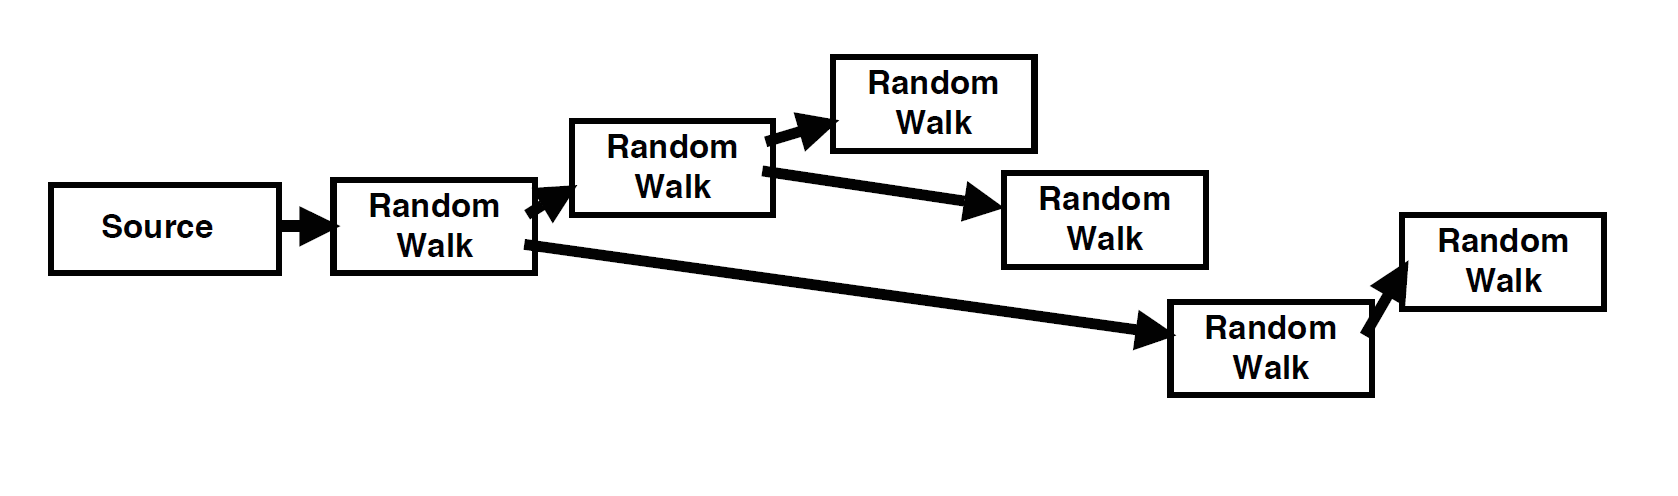
\includegraphics[width=0.85\textwidth]{walkE.png}
\caption{MCNP random walk.}
\label{fig:randomwalk}
\end{figure}
For example, the collision angle and change of speeds will be different at every simulation run. The underlying assumption here is that eventually, after many samples (on the order of magnitude of 100,000) the results will converge to the actual value. Another way to look at this is a coin toss problem. If one tosses a coin, it's evident that the probability of getting a head is the same as of getting a tail - 50\%. However, after 10 tosses, the coin may not have landed on its head 5 times and on its tail 5 times. However, as one starts tossing the coin 100 times, or 1,000 times, the results will distribute themselves more evenly - converging towards the 50-50 split of heads and tails. This is the exact same approach used in Monte Carlo simulations. Encompassing these random samples and properties of various materials is MCNP, or Monte Carlo N-Particle Transport Code.

\subsubsection{MCNP}
The Monte Carlo N-Particle Transport Code was developed by the Los Alamos National Laboratory in the 1950s. Primarily, it is used to simulate nuclear processes, such a fission. Other applications It is ideal for this project since the main reaction used is fission in the novel reactor. There have been several versions of MCNP released over the years, with further improvements to its vast materials library. The library contains information of physical properties like melting and boiling points of materials, as well as more advanced aspects like neutron capturing properties and atomic cross sectional areas. Version 5.1 and X were used for the design and simulation of the Geometrically Optimized Flux Reactor (GOFR). In order to simulate any particle interactions, MCNP solves the Boltzmann transport equation, defined as:
\begin{equation}
\Psi(\vec{r},\vec{v}) = \int\Big(\int\Psi(\vec{r'},\vec{v'})C(\vec{v'}\rightarrow \vec{v},\vec{r'})d\vec{v'} + Q(\vec{r'},\vec{v})\Big)T(\vec{r'}\rightarrow \vec{r},\vec{v})d\vec{r'}
\end{equation}
The $\Psi(\vec{r},\vec{v})$ term defines the collision density of particles across the whole simulation space. The $C$ is called the collision kernel, which accounts for particles changing their velocity at a given location. The $T$ term, on the other hand, is the transport kernel and accounts for the opposite case - a particle changing its location at a given velocity. The $Q$ term is the source of particles. In the case of GOFR, the term is defined as:
\begin{equation}
Q(r,v) = S(\vec{r},\vec{v}) + \int\Psi(\vec{r},\vec{v'})F(\vec{v'}\rightarrow \vec{v},\vec{r})d\vec{v'}
\end{equation}
$S$ defines the fact that the source is stationary, and that the primary particles will be emitted from a fixed point in the simulation space. The collision density term accounts for the fact that the core will be undergoing fission, defined as $F$. What makes MCNP so powerful is the simultaneous use of the collision and transport kernels. Taking both factors into account allows the simulation to look at particles that change velocity and direction at any point in the simulation space. Every interaction that a particle has with another particle is stored in the simulation memory. The states of the particles - energy, velocity, direction - are saved in order to extrapolate results and determine the convergence. The flow diagram in Figure \ref{fig:randomwalk}, can also be seen in terms of particle histories, seen in Figure \ref{fig:histories}.

\begin{figure}[!htbp]
\centering
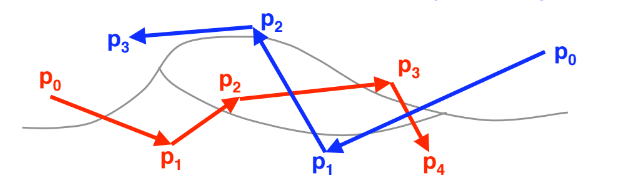
\includegraphics[width=0.85\textwidth]{histories.png}
\caption{Particle interaction histories.}
\label{fig:histories}
\end{figure}
With the histories, MCNP is able to extrapolate where the particles will end up after future runs and what their energies will be. The final results are defined in the following way:
\begin{equation*}
A = \int A(p)\Psi(p)dp \approx \frac{1}{M}\sum_{m=1}^M\Big(\sum_{k=1}^\infty A(p_{k,m})\Big)
\end{equation*}
The final, average state of the particle is the integral of the product between the collision density and the particle states. The integral can be estimated through a classic Riemann sum, where $M$ is the number of particle histories and samples. The larger the value of $M$, the more accurate the final results are. 

Through the extensive calculations that MCNP carries out, the decades of development put into it, as well as its ability to take into account all physical properties of materials used, the software package proved ideal for the design and simulation of the Geometrically Optimized Flux Reactor (GOFR).
